%\PassOptionsToPackage{demo}{graphicx}
\PassOptionsToPackage{table}{xcolor}
\documentclass[portrait,final,a0paper,fontscale=0.320]{imiseposter}
\usepackage[utf8]{inputenc}
\usepackage[english]{babel}
\usepackage[T1]{fontenc}

\usepackage{tcolorbox}
\usepackage{relsize}
%\usepackage[breaklinks=true]{hyperref}% hyperref links are displaced with baposter because of the font scale 
\usepackage{url}
\usepackage{graphicx}
\usepackage{multicol}
\usepackage{siunitx}
\usepackage{booktabs}
\usepackage{tabulary}
\usepackage{cleveref}

\usepackage{listings}
\lstset{
 columns=fullflexible,
%  frame=single,
 breaklines=true,
 breakatwhitespace=true,
% basicstyle=\ttfamily
%  postbreak=\mbox{\textcolor{red}{$\hookrightarrow$}\space},
}
\lstset{language=SQL,morekeywords={minus,ask,bb,meta,rdfs,skos}}

%\usepackage{times}
%\usepackage{helvet}
%\usepackage{bookman}
\usepackage{palatino}
\renewcommand{\familydefault}{\sfdefault}

\newcommand{\captionfont}{\footnotesize}
\usepackage[font=small,labelfont=bf]{caption}


%%%%%%%%%%%%%%%%%%%%%%%%%%%%%%%%%%%%%%%%%%%%%%%%%%%%%%%%%%%%%%%%%%%%%%%%%%%%%%
%%% Begin of Document
%%%%%%%%%%%%%%%%%%%%%%%%%%%%%%%%%%%%%%%%%%%%%%%%%%%%%%%%%%%%%%%%%%%%%%%%%%%%%%

\begin{document}

%%%%%%%%%%%%%%%%%%%%%%%%%%%%%%%%%%%%%%%%%%%%%%%%%%%%%%%%%%%%%%%%%%%%%%%%%%%%%%
%%% Here starts the poster
%%%---------------------------------------------------------------------------
%%% Format it to your taste with the options
%%%%%%%%%%%%%%%%%%%%%%%%%%%%%%%%%%%%%%%%%%%%%%%%%%%%%%%%%%%%%%%%%%%%%%%%%%%%%%
% Define some colors

% Corporate design colors of the medical faculty of the Uni of Leipzig, new design of 2018
%\definecolor{lowertriangle}{RGB}{9,65,81}

%%
\begin{poster}% Set grid to false for final print
  {grid=true,}
  % Eye Catcher
  {
\includegraphics[width=30em]{img/medfak.pdf}} 
  % Title
  {\bf\textsc{Linked Open Data about Management of Health Information Systems}\vspace{0.5em}
  }
  % Authors
  {\textsc{Konrad Höffner\footnote{konrad.hoeffner@imise.uni-leipzig.de}, Franziska Jahn, Anna Lörke, Thomas Pause, Birgit Schneider, Elske
  Ammenwerth, Alfred Winter}}
  % University logo
  {% The makebox allows the title to flow into the logo, this is a hack because of the L shaped logo.
    %
\includegraphics[height=9.0em]{img/medfak.pdf}
  }


%%%%%%%%%%%%%%%%%%%%%%%%%%%%%%%%%%%%%%%%%%%%%%%%%%%%%%%%%%%%%%%%%%%%%%%%%%%%%%
%%% Now define the boxes that make up the poster
%%%---------------------------------------------------------------------------
%%% Each box has a name and can be placed absolutely or relatively.
%%% The only inconvenience is that you can only specify a relative position 
%%% towards an already declared box. So if you have a box attached to the 
%%% bottom, one to the top and a third one which should be in between, you 
%%% have to specify the top and bottom boxes before you specify the middle 
%%% box.
%%%%%%%%%%%%%%%%%%%%%%%%%%%%%%%%%%%%%%%%%%%%%%%%%%%%%%%%%%%%%%%%%%%%%%%%%%%%%%
    %
    % A coloured circle useful as a bullet with an adjustably strong filling
    \newcommand{\colouredcircle}{%
      \tikz{\useasboundingbox (-0.2em,-0.32em) rectangle(0.2em,0.32em); \draw[draw=black,fill=imiseblue,line width=0.03em] (0,0) circle(0.18em);}}

%%%%%%%%%%%%%%%%%%%%%%%%%%%%%%%%%%%%%%%%%%%%%%%%%%%%%%%%%%%%%%%%%%%%%%%%%%%%%%
\begin{posterbox}[name=background,column=0,row=0]{Background}

%\begin{minipage}{\linewidth}
%\centering
%\captionof{figure}{The SNIK Meta Model}
%\label{fig:metamodel}
%\end{minipage}
The Semantic Network of Information Management in Hospitals (SNIK) is an OWL 2 DL ontology with a modular architecture:
The meta model provides a common vocabulary for the domain of hospital information system (HIS) management.
% and thus defines, which superclasses and relations can be used., see \cref{fig:metamodel}.
It defines three basic disjunctive classes: Role (who), Function (does what) and Entity Type (which information is read and written). %, see \cref{fig:metamodel}.
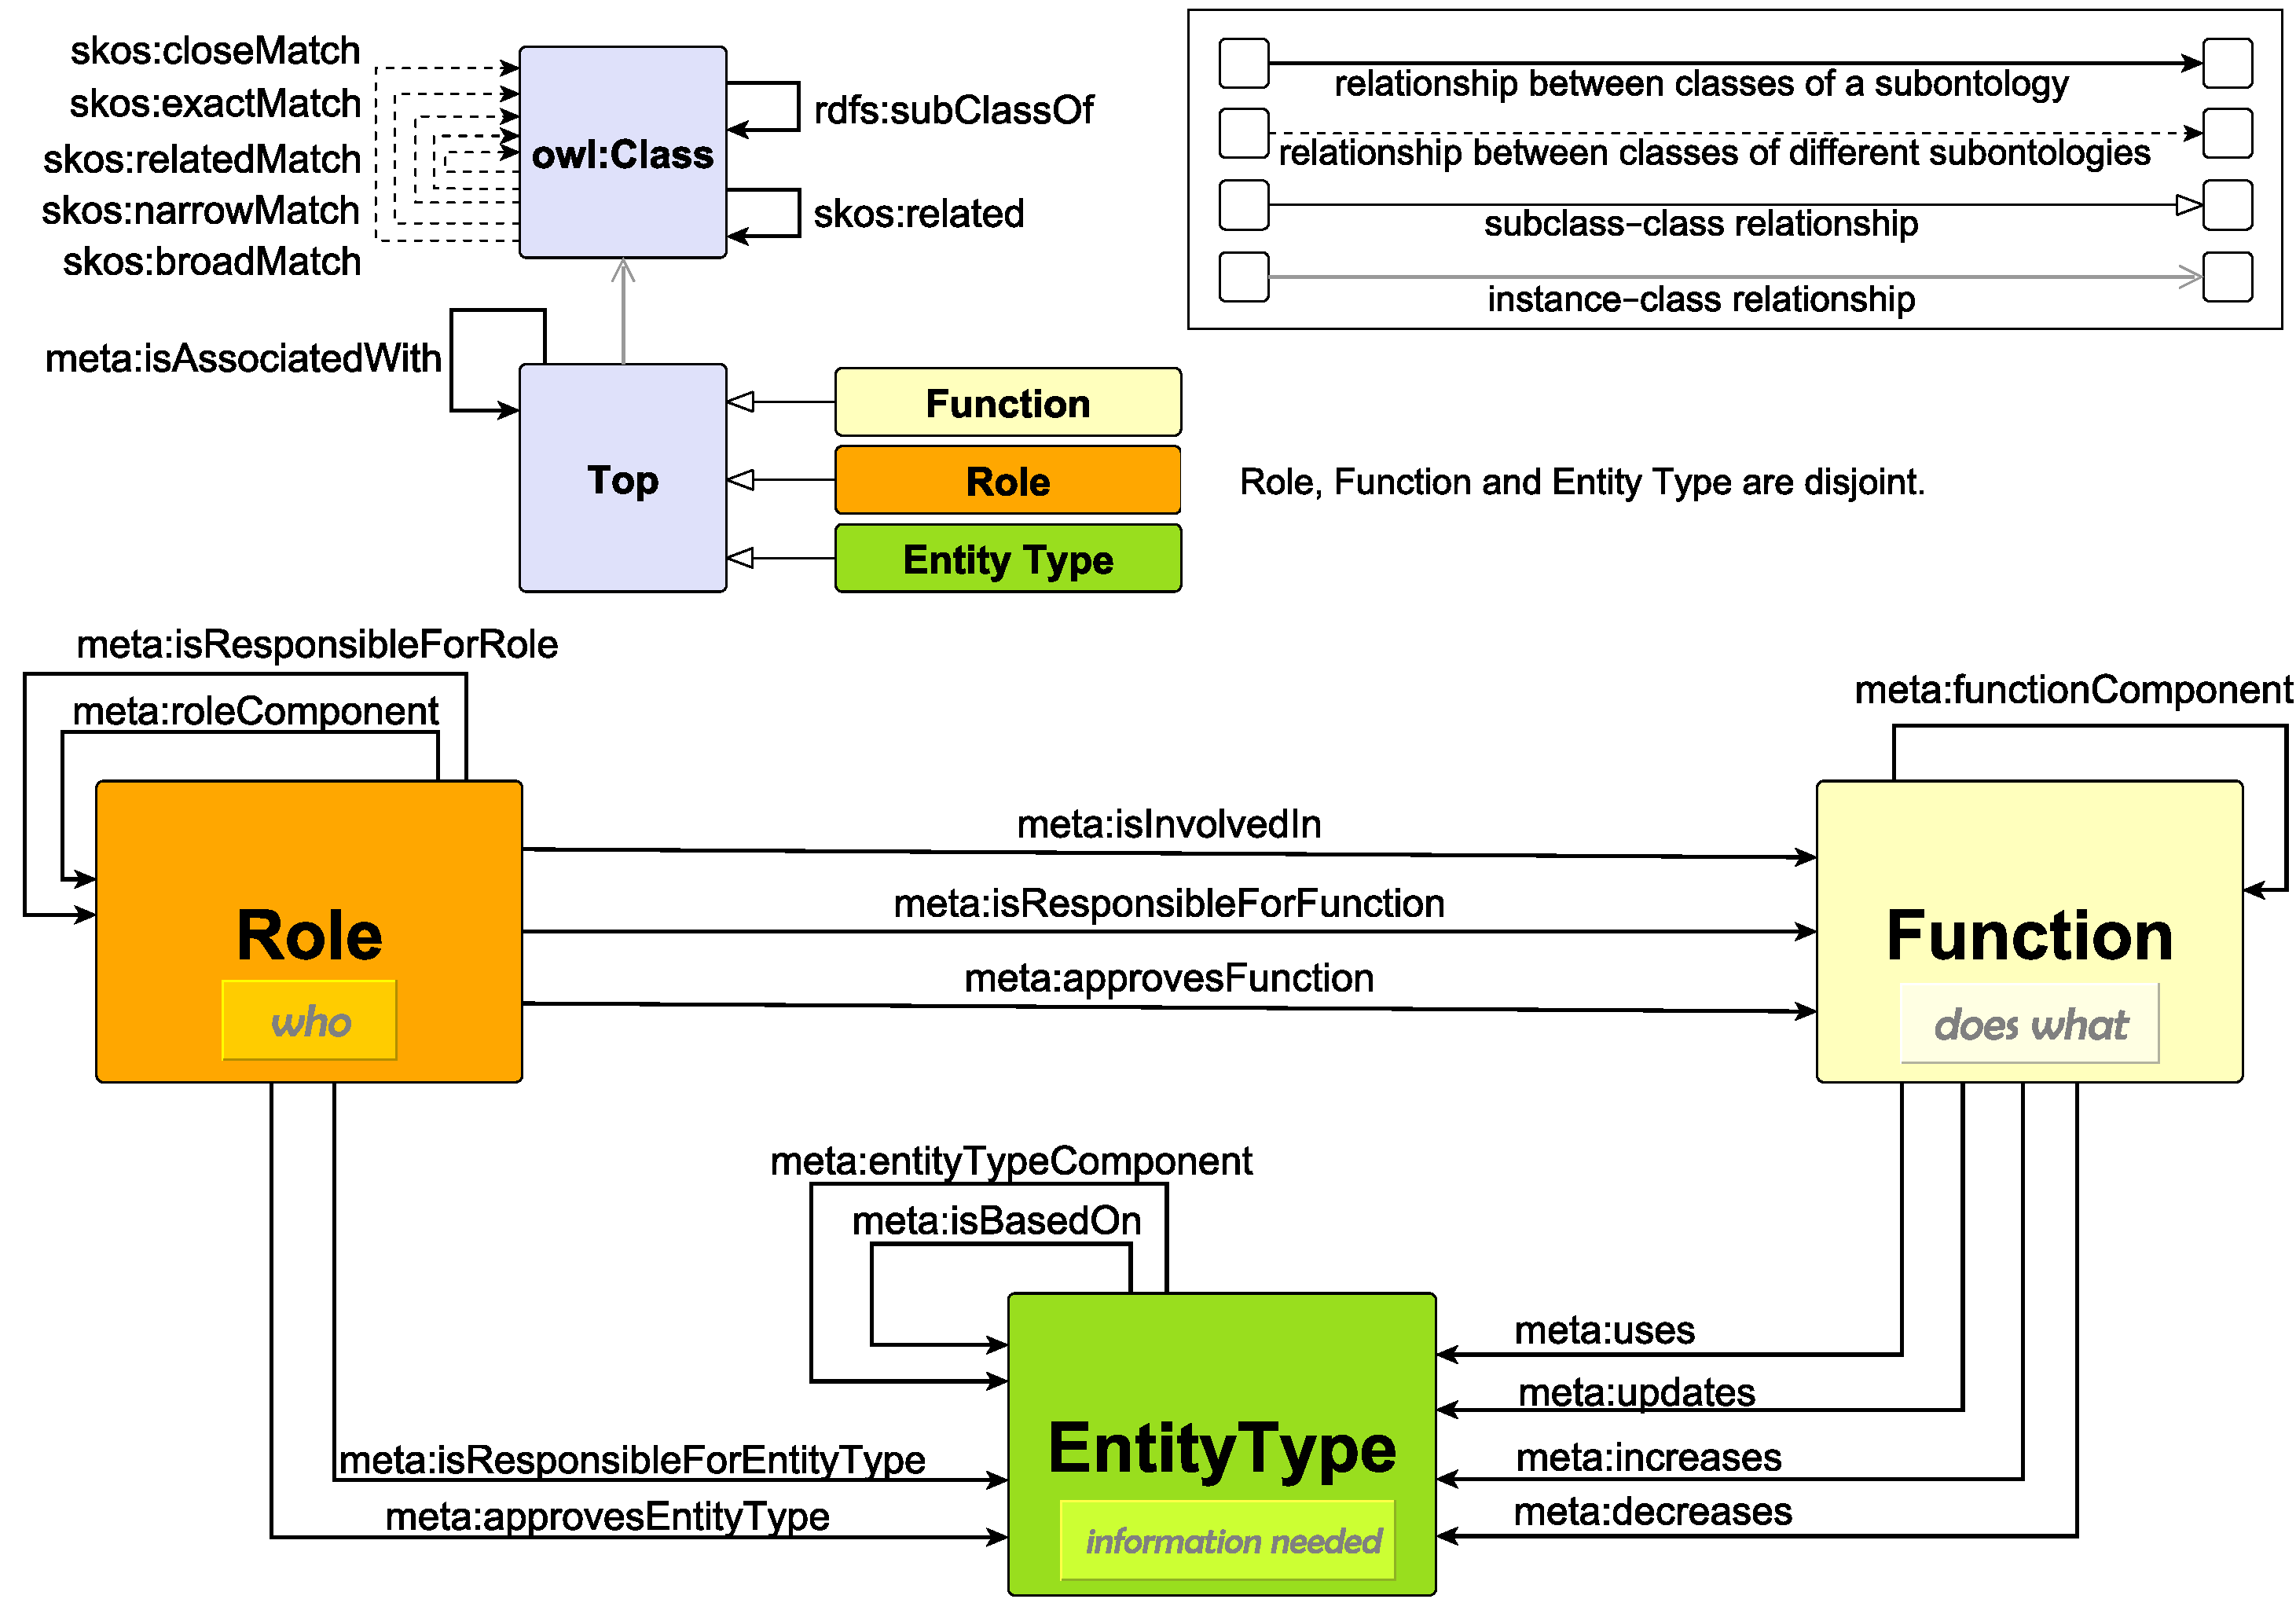
\includegraphics[width=1.01\columnwidth]{img/metamodel9s.pdf}
\vspace{0.3em}
\end{posterbox}
%%%%%%%%%%%%%%%%%%%%%%%%%%%%%%%%%%%%%%%%%%%%%%%%%%%%%%%%%%%%%%%%%%%%%%%%%%%%%%
\begin{posterbox}[name=methods,below=background]{Methods}
Semantic Web technologies principles are used to create, store and publish SNIK as Linked Open Data~\cite{sniktec}.
Subontologies are manually extracted from different sources and build upon the meta model by attaching their subclass hierarchies to the Function, Role and EntityType classes.
{\centering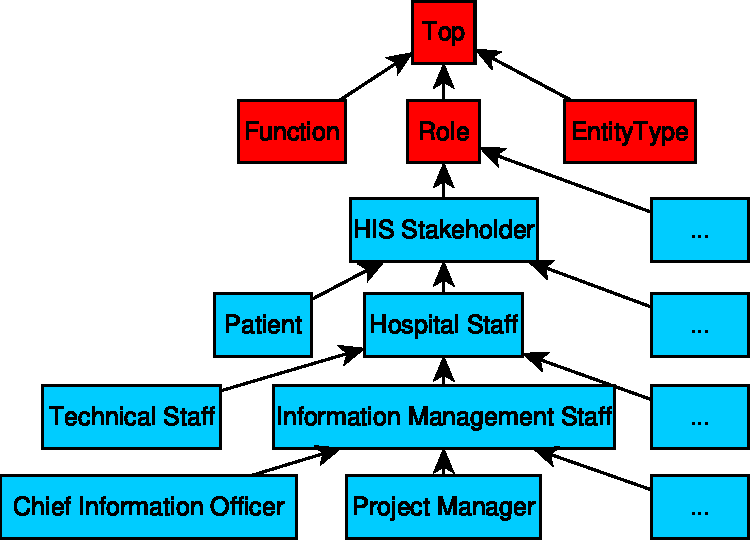
\includegraphics[width=0.8\columnwidth]{img/hierarchy.pdf}}
\begin{center}
\begin{tabular*}{0.96\columnwidth}{lll}
\toprule
\textbf{Ontology}				&\textbf{Prefix}&\textbf{Source}\\
\midrule
\url{http://www.snik.eu/ontology/meta}		&meta		&All Sources\\
\url{http://www.snik.eu/ontology/bb}		&bb		&Textbook~\cite{bb}\\
\url{http://www.snik.eu/ontology/ob}		&ob		&Textbook~\cite{ob}\\
\url{http://www.snik.eu/ontology/he}		&he		&Textbook~\cite{he}\\
\url{http://www.snik.eu/ontology/ciox}		&ciox		&CIO Interview\\
\url{http://www.snik.eu/ontology/it4it}		&it4it		&Standard~\cite{it4it}\\
\bottomrule
\end{tabular*}
\end{center}

%inked Data principles, each class of SNIK has a unique URL.
%resource using the HTTP protocol to receive a description of
%the class, respectively the concept being represented by the
%class, using the standards RDF and SPARQL. Opening a
%We show that those interfaces can benefit teaching, system analysis and integration.
\end{posterbox}
%%%%%%%%%%%%%%%%%%%%%%%%%%%%%%%%%%%%%%%%%%%%%%%%%%%%%%%%%%%%%%%%%%%%%%%%%%%%%%
\begin{posterbox}[name=results,column=1]{Results}
SNIK v0.8 contains \num{4729} classes, \num{329} properties, \num{713} interlinks and \num{112747} triples and is available under the CC BY-NC-SA 4.0 as:
\iffalse
\begin{tabulary}{\columnwidth}{lL}
\toprule
%URL		&\url{http://www.snik.eu/ontology}\\
RDF dump	&\url{https://github.com/IMISE/snik-ontology/releases/download/0.8.0/snik-0.8.zip}\\
LodLive Browser	&\url{http://www.snik.eu/ontology}\\
SNIK Graph	&\url{http://www.snik.eu/graph}\\
SPARQL Endpoint	&\url{http://www.snik.eu/sparql}\\
%RDF Dump	&\url{https://github.com/IMISE/snik-ontology/releases/download/0.8.0/snik-0.8.zip}\\
\bottomrule
\end{tabulary}%The source code for the services is available at \url{https://github.com/imise}
\fi
%The \emph{RDF dump} is available at \url{https://github.com/IMISE/snik-ontology/releases/download/0.8.0/snik-0.8.zip} and contains all triples of SNIK in Turtle syntax, such as:

%\begin{tcolorbox}[colback=white,colframe=mediblue,title=RDF Dump\\\url{https://github.com/IMISE/snik-ontology/releases/download/0.8.0/snik-0.8.zip}]
\begin{tcolorbox}[colback=white,colframe=mediblue,title=RDF Dump~~\url{http://www.snik.eu/download/snik-0.8.zip}]
The \emph{RDF dump} contains all triples of SNIK in Turtle syntax, such as:
\begin{lstlisting}[basicstyle=\ttfamily]
bb:InformationSystem
        rdfs:label "Information System"@en;
        rdfs:subClassOf bb:InformationManagementEntityType;
        skos:closeMatch ob:InformationSystem;
        meta:supports bb:Documentation.
\end{lstlisting}
%offers several interfaces that are useful for researchers practitioners and students, depending on their objectives and their semantic web skills.
\vspace{-1.0em}
\end{tcolorbox}
\vspace{-0.5em}

\begin{tcolorbox}[colback=white,colframe=mediblue,title=LodLive RDF Browser~~~~~~~~~~~~~\url{http://www.snik.eu/ontology}]
%Users can open a SNIK class URL in a web browser using \emph{LodLive}~\cite{lodlive}:
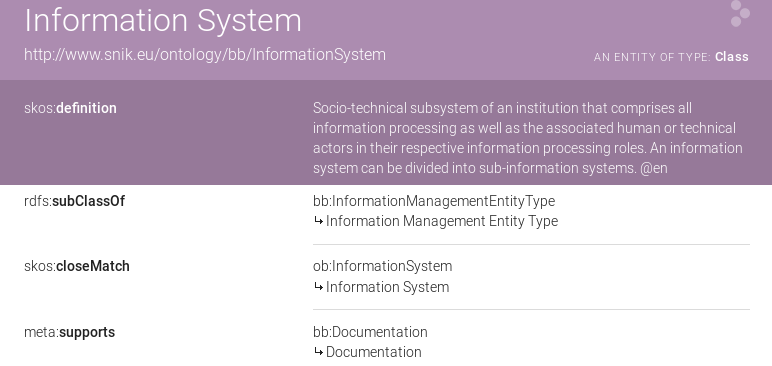
\includegraphics[width=\textwidth]{img/lodlive.png}
\vspace{-1.0em}
\end{tcolorbox}
\vspace{-0.5em}

\begin{tcolorbox}[colback=white,colframe=mediblue,title=SNIK Graph~~~~~~~~~~~~~~~~~~~~~~~~~~~~~~\url{http://www.snik.eu/graph}]
\emph{SNIK Graph} visualizes the structure of SNIK by modelling each class as a node and each RDF triple and OWL restriction as an edge:
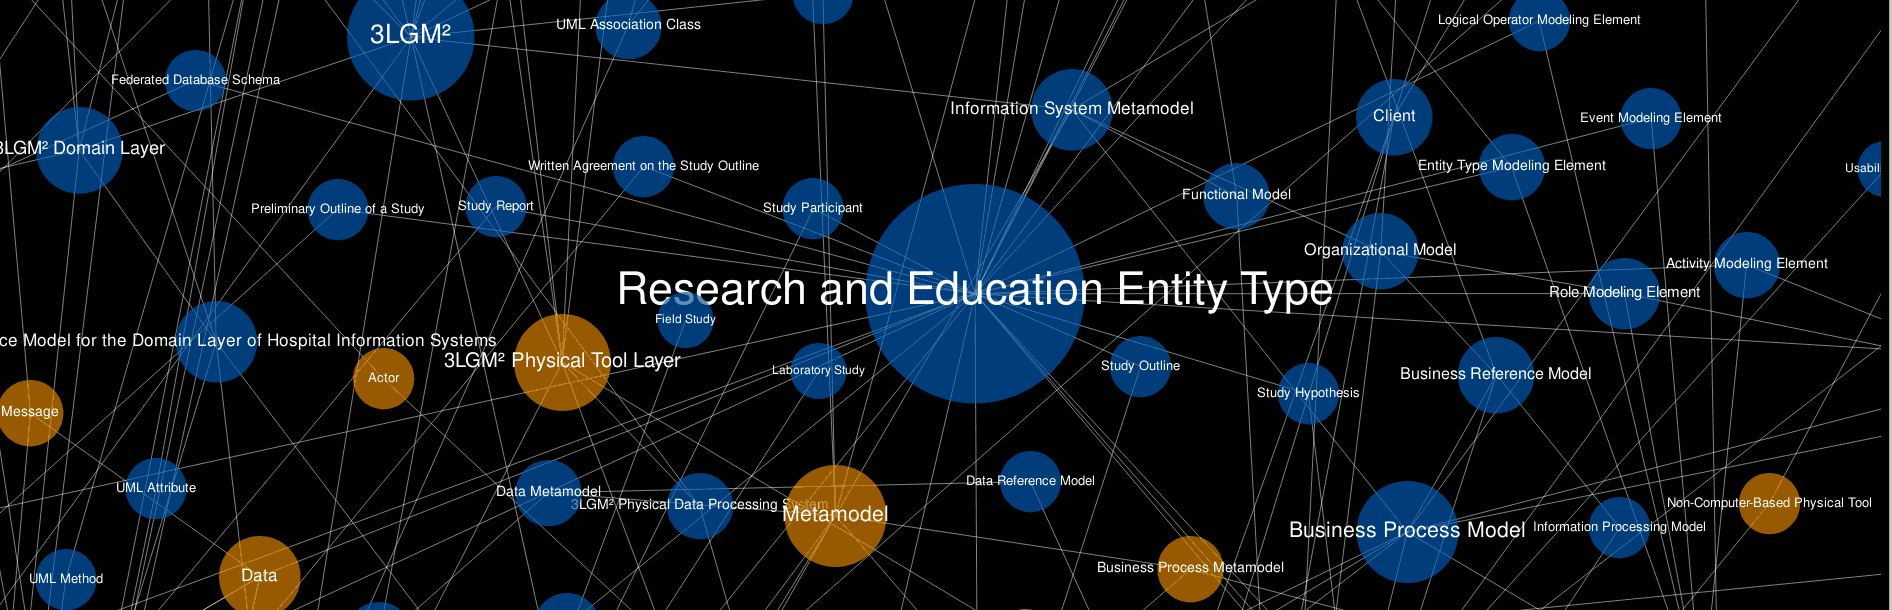
\includegraphics[width=\textwidth]{img/snikgraph.png}
%SNIK Graph queries the list of classes and their relations from the SPARQL endpoint and transforms them into nodes and edges of the graph.
%Exploration options like the “spider worm”, which consists of the shortest path between a start node and an end node together with the end node’s neighbourhood, illustrate the context of a concept.
%The meta model and the subontologies can be freely accessed via SPARQL queries:
\vspace{-1.0em}
\end{tcolorbox}
\vspace{-0.5em}

\begin{tcolorbox}[colback=white,colframe=mediblue,title=SPARQL Endpoint~~~~~~~~~~~~~~~~\url{http://www.snik.eu/sparql}]
The SPARQL endpoint is the most expressive interface to SNIK but requires knowledge of both the SPARQL syntax and the SNIK meta model.
%Read access is publicly available at \url{http://www.snik.eu/sparql} 
It can be used both as an API and directly. Examples:\\

Which healthcare network components are not healthcare institutions?
\begin{lstlisting}
SELECT ?x {bb:HealthCareNetwork meta:entityTypeComponent ?x.
  MINUS {?x rdfs:subClassOf* bb:HealthCareInstitution.}}
\end{lstlisting}
How many functions is the CIO responsible for?
\begin{lstlisting}
SELECT COUNT(?f) {bb:ChiefInformationOfficer meta:isResponsibleForFunction ?f.}
\end{lstlisting}
%
%Do transinstitutional health information systems support telemicroscopy?
%\begin{lstlisting}
%ASK {bb:TransinstitutionalHealthInformationSystem meta:supports bb:Telemicroscopy.}
%\end{lstlisting}
\vspace{-1.0em}
\end{tcolorbox}
\vspace{-0.5em}

\end{posterbox}
%%%%%%%%%%%%%%%%%%%%%%%%%%%%%%%%%%%%%%%%%%%%%%%%%%%%%%%%%%%%%%%%%%%%%%%%%%%%%%
\begin{posterbox}[name=discussion,column=1,below=results]{Discussion}
SNIK is published using open standards over interfaces with different compromises between expressivity and accessibility for different audiences.
Future work includes a dedicated ontology modelling tool.
%Different user groups can use the interfaces of SNIK that are most suitable to them:
%For example, the IT management of a hospital can use SNIK as a vocabulary to integrate data from different formats that result from application components from different vendors.
%Using the SPARQL query language, experts can also integrate applications with the SNIK ontology.
%Experts can also use the SPARQL query editor to answer specific questions.
%Students and teachers benefit more from SNIK Graph and the RDF browser, which intuitively presents knowledge without the need for technical skills.
\begin{center}
\begin{tabulary}{\textwidth}{lll}
\toprule
\textbf{Goal}		&\textbf{Audience}		&\textbf{Interfaces}\\
\midrule
Teaching	&Teachers and Students		&SNIK Graph, LodLive\\
Integration	&Hospital Management		&SPARQL Endpoint, RDF Dump\\
Modelling	&Experts, Ontologists		&SPARQL Endpoint, RDF Dump\\
\bottomrule
\end{tabulary}
\end{center}

\begin{tabulary}{\columnwidth}{lL}
\toprule
\bottomrule
\end{tabulary}%The source code for the services is available at \url{https://github.com/imise}

\end{posterbox}
%%%%%%%%%%%%%%%%%%%%%%%%%%%%%%%%%%%%%%%%%%%%%%%%%%%%%%%%%%%%%%%%%%%%%%%%%%%%%%
\begin{posterbox}[name=references,column=0,below=methods]{References}
    \smaller
    \bibliographystyle{abbrv}
    \begingroup
    \renewcommand{\section}[2]{}%suppress heading
    \bibliography{poster}
    \endgroup
    \vspace{0.3em}
    %The SNIK project is supported by the DFG (German Research Foundation) under the grant numbers 1605/7-1 and 1387/8-1.
    SNIK is supported under the DFG grant numbers 1605/7-1 and 1387/8-1.
  \end{posterbox}
%%%%%%%%%%%%%%% IMISE Logo
 \node [anchor=north east, inner sep=1pt,yshift=-2em,xshift=-1em] at (current page.north east)
 {
\includegraphics[height=0.03\textheight]{img/imise-logo.pdf}
 };
%%%%%%%%%%%%%%% SNIK Logo 
 \node [anchor=south east, inner sep=1pt,xshift=-35em] at (current page.south east) % for unknown reasons the xshift is necessary
 {
\includegraphics[height=0.03\textheight]{img/snik-logo.png}
 };
%%%%%%%%%%%%%%% DFG Logo
 \node [anchor=south east, inner sep=1pt,xshift=-2.5em] at (current page.south east) % for unknown reasons the xshift is necessary
 {
\includegraphics[height=0.03\textheight]{img/dfg-logo.pdf}
 };
%%%%%%%%%%%%%%%%%%%%%%%%%%%%%%%%%%%%%%%%%%%%%%%%%%%%%%%%%%%%%%%%%%%%%%%%%%%%%%
\end{poster}
\end{document}

